\documentclass[a4paper, 11pt]{article}
\usepackage[slovene]{babel}
\usepackage[utf8]{inputenc}
\usepackage[T1]{fontenc}
\usepackage{amsfonts,amsmath,amssymb}
\usepackage{amsthm}
\usepackage{amsmath}
\usepackage{amssymb}
\usepackage{graphicx}

\newtheorem{Izrek}{Izrek}

\begin{document}

\begin{titlepage}
    \begin{center}
        \LARGE
        UNIVERZA V LJUBLJANI\\
        FAKULTETA ZA MATEMATIKO IN FIZIKO\\
        FINANČNA MATEMATIKA\\

        \vspace*{5cm}
        
        Finančni praktikum\\
        \huge
        \textbf{The power of two or more choices}

        \vspace*{6cm}

        \Large
        Avtorja:\\
        Nejc Kumer in Neža Lesnjak
    \end{center}
\end{titlepage}

\tableofcontents
\pagebreak

\section{Navodila}

Imamo $n$ žog in $n$ košev. Žoge polagamo v koše na spodnje načine:

\begin{itemize}
    \item za vsako žogo izberemo naključen koš in žogo vržemo vanj.
    \item za vsako žogo naključno izberemo dva izmed košev in žogo vržemo v tistega, 
    ki smo ga do tega trenutka manjkrat zadeli.
    \item za vsako žogo naključno izberemo tri izmed košev in žogo vržemo v tistega, 
    ki smo ga do tega trenutka manjkrat zadeli.
    \item ...
\end{itemize}

Zanima nas maksimalna zasedenost, torej število zadetkov v tisti koš, ki smo ga največkrat zadeli.
Eksperimentalno analizirajte te naključne postopke.\\
Kaj se zgodi, če imamo $n$ košev in $2n$, $3n$, $4n$ ... žog?
V tem primeru nas zanima tudi minimalna zasedenost.
Za $n$ izbiramo velike vrednosti.

\section{Opis problema}

Problem $n$ žog in $n$ košev je v teoriji verjetnosti znan problem, ki ima veliko aplikacij tudi v drugih vedah, predvsem v računalništvu.\\
Delitev žog v koše je lahko popolnoma naključna ali delno naključna.
V zgoraj naštetih primerih delitve gre le v prvi točki za popolnoma naključno delitev.
V vseh naslednjih točkah imamo delno naključno delitev - naključno izberemo le določeno število košev in nato žogo položimo v tistega izmed izbranih,
ki smo ga do tega trenutka najmanjkrat zadeli. To v angleškem jeziku poimenujemo \emph{the power of
two or more choices} - odvisno od tega, koliko košev naključno izberemo.

\section{Pričakovani rezultati}

Če imamo torej $n$ košev in $n$ žog v prvem delu naloge, ko za vsako žogo naključno izberemo koš in vržemo žogo vanj,
za koš z največ žogami pričakujemo rezultat iz spodnjega izreka.

\begin{Izrek}
    Koš z največ žogami ima $\Omega (\frac{\log{n}}{\log{\log{n}}})$ žog z verjetnostjo $1 - \frac{1}{\sqrt[3]{n}}$.
\end{Izrek}

V drugem delu naloge, torej v primeru, ko naključno izberemo $d$ košev (in $d \geq 2$), ter žogo položimo v bolj praznega od njih,
pa bomo pričakovali spodnji rezultat.

\begin{Izrek}
    Koš z največ žogami ima $\frac{\log {\log{n}}}{\log{d}} + O(1)$ žog z verjetnostjo blizu 1.
\end{Izrek}

Rezulata iz slednjega izreka je skoraj eksponentno manjši kot rezultat iz prvega izreka za popolnoma naključno delitev žog v koše.

V nalogi bova preverila, kako se rezultati maksimalne zasedenosti spreminjajo, če žoge razporejamo na različne, zgoraj omenjene načine
in kako, če imamo $n$ košev in $n$, $2n$, $3n$, ... žog.


\section{Programiranje rešitev}

Najprej sva pripravila funkcijo, ki kot argumente sprejme
število žog $n$, število košev $N$, ter število $d$, ki pove,
med koliko koši izbiramo. 
Kot argument prejme tudi $stevilo$ $ponovitev$, iz katerega se nato izračuna povprečen rezultat.

Funkcija beleži skupen čas trajanja. 

S pomočjo ukaza \emph{random} za vsako izmed
žog izbere naključnih $d$ košev.
Nato s pomočjo funkcije \emph{argmin} - ki sva jo definirala tako,
da iz seznama košev določi tisto mesto na seznamu, na katerem je koš, v katerem je najmanj žog - 
določimo, v katerega izmed $d$ košev bomo vrgli žogo.

Rezultati maksimalne zasedenosti iz vsake ponovitve se beležijo in na koncu se izračuna 
povprečno največje število žog v najbolj zasedenem košu.
Poleg tega funkcija vedno izračuna še analitičen rezultat,
ki določa spodnjo mejo zasedenosti.

Funkcija poleg zgoraj omenjenega povprečnega in analitičnega rezultata
vrne kot rezultat tudi čas trajanja izvedbe posamezne ponovitve.

\begin{verbatim}
    def najvecje_stevilo_zog_v_kosu(N,n,d,stevilo_ponovitev):
        max_zasedenosti = []
        kosi = range(N)
        start = time.time() 
        for ponovitev in range(stevilo_ponovitev):
            zoge = [0] * N       
            for i in range(n):
                kateri = random.sample(kosi, d) 
                koliko = [zoge[j] + (random.randint(0, 25) / 100) 
                          for j in kateri]    
                k = argmin(koliko)      
                zoge[kateri[k]] += 1    
           max_zasedenosti.append(max(zoge))   
        end = time.time() 
        avg = sum(max_zasedenosti)/len(max_zasedenosti) 
        if d == 1:
            analiticno = log(n)/log(log(n)) 
        else:
            analiticno = log(log(n))/log(d) 
        return avg, analiticno, end-start
\end{verbatim}

Nato pa sva definirala še funkcijo:

\begin{verbatim}
    def izvedi_funkcijo(Poskusi, N, n, d, stevilo_ponovitev):
        print("izvedi_funkcijo(%d, %d, %d, %d, %d)" % 
                        (Poskusi, N, n, d, stevilo_ponovitev))
        ime_datoteke = "najvecja_zasedenost_%d_%d_%d.csv" % (N, n, d)
        with open(ime_datoteke, "w") as f: 
            wr = csv.writer(f)
            wr.writerow(["avg", "analiticno", "cas"])
            # Ce je Poskusi == 0 izvajamo do prekinitve, sicer omejeno
            i = 0
            if Poskusi == 0:
                Poskusi = -1
            while i != Poskusi:
                avg, analiticno, cas = 
                    najvecje_stevilo_zog_v_kosu(N, n, d, stevilo_ponovitev)
                avg = round(avg, 4)
                analiticno = round(analiticno, 4)
                wr.writerow([avg, analiticno, cas])
                f.flush() 
                i += 1
\end{verbatim}

Ta funkcija kot argument sprejme \emph{Poskusi} - število poskusov, poleg tega pa še enake argumente kot prva funkcija. 
Ta funkcija ustvari \emph{csv} datoteko, v katero nato po vrsticah
zapisuje rezultate prve funkcije, ki jo pokliče tolikokrat,
kot določimo v argumentu \emph{Poskusi}. 

\pagebreak


\section{Analiza rezultatov}

\subsection{Popolnoma naključna delitev žog in $N = n$}
Rezultati popolno naključnega razporejanja žog, pri enakem številu košev in žog.
Predstavljeni so rezultati za $n = N = 1000$, $n = N = 10000$ in $n = N = 100000$.

Z rdečo črto so označene povprečne vrednosti, in iz njih sklepava, da za različne $n$ (ki so 
oblike $10^x$) velja,
da je največje število žog v košu približno enako $1,1(2+log(n))$.

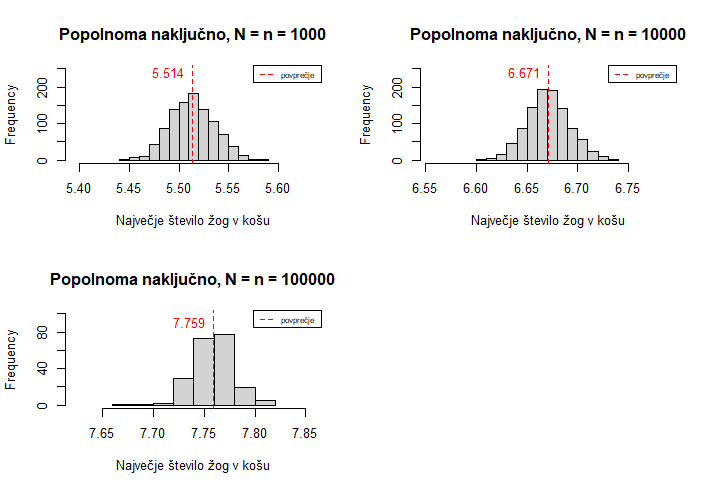
\includegraphics[scale=0.6]{popolnoma_nakljucno.png}

\subsection{Delno naključna delitev žog in $N = n$}

Spodaj so prikazani rezultati delno naključne delitve za $d=2$ in $d=4$, pri čemer imamo
$N = n = 10000$. 

Za primerjavo je dodana tudi popolnoma naključna delitev žog, torej za $d = 1$.

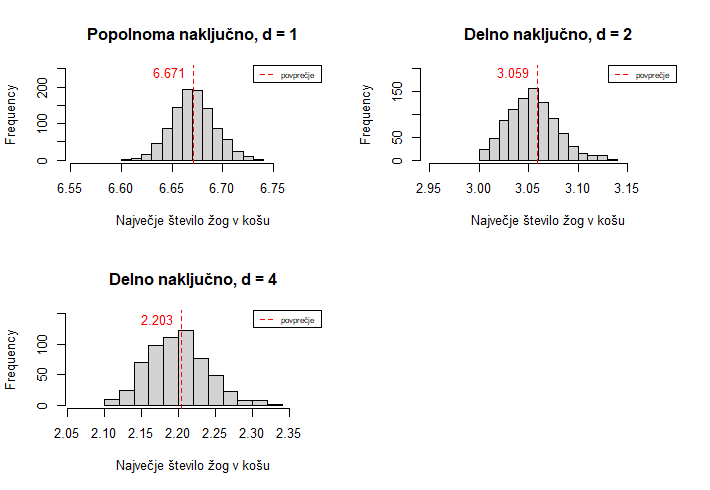
\includegraphics[scale=0.6]{delno_nakljucno.png}

\subsection{$n$ košev in $n$, $2n$, $3n$ žog}

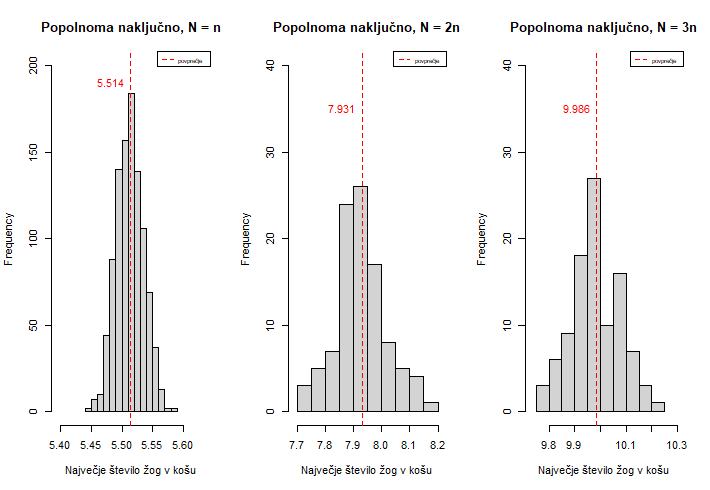
\includegraphics[scale=0.60]{popolnoma_nakljucno2.png}

Najprej imamo zgoraj rezultate, ko žoge razporejamo popolnoma naključno.
Predstavljeni so primeri, ko imamo $1000$ košev in $1000$, $2000$ ter $3000$ žog.
\\
\\
Spodaj pa imamo primere za $1000$ košev in $1000$, $2000$ ter $3000$ žog, pri čemer žoge 
razporejamo delno naključno z $d = 2$. 

Sklepava, da v primerih, ko velja $d = 2$ in $n = 1000$, za največje število žog v košu približno
velja vrednost $log(n) + \frac{N}{n} -1$. 

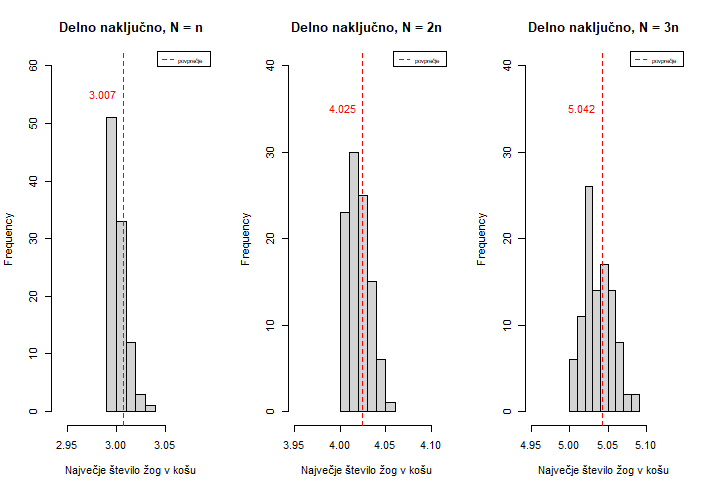
\includegraphics[scale=0.60]{delno_nakljucno2.png}

\subsection{Časovna odvisnost}

V spodnjih tabelah je prikazan povprečni čas, ki je potreben za izvedbo ene ponovitve poskusa za določene podatke. 

Pri prvi tabeli smo primerjali časovno zahtevnost algoritma za različno število naključno izbranih košev - različne $d$. 
Ugotovili smo, da z večanjem naključnega števila izbranih košev linearno narašča tudi čas, 
ki je potreben za izvedbo našega algoritma, in sicer za vsak povečan $d$, se čas izvajanja algoritma podaljša za približno sekundo.

\begin{center}
    \begin{tabular}{|c|c|}
        \hline
        $d$ & čas \\
        \hline
        2 & 6.649257 \\
        \hline
        3 & 8.275287 \\
        \hline
        4 & 9.931728 \\
        \hline
        5 & 11.616240 \\ 
        \hline
    \end{tabular}
\end{center}

Rezultati spodnje tabele, kjer imamo povprečno časovno zahtevnost algoritma glede na število vseh košev in žog v poskusu, so precej podobni rezultatom iz prve tabele - spet se pojavi linearno naraščanje. 

Opazimo lahko, da se za vsakih $1000$ novih obravnavanih košev, izvajanje našega algoritma podaljša za približno $5$ sekund. 

\begin{center}
    \begin{tabular}{|c|c|}
        \hline
        št. košev/žog & čas \\
        \hline
        1000 & 5.00000 \\
        \hline
        10000 & 50.07592 \\
        \hline
        100000 & 498.73500 \\
        \hline
    \end{tabular}
\end{center}

\pagebreak
\section{Literatura}

https://en.wikipedia.org/wiki/Balls\_into\_bins\_problem

\end{document}